%TC: macro \marginfootnote [other]
%TC: envir SCfigure [] other
%TC: macrocount beginSCfigure [figure]
\documentclass[11pt]{report}
\usepackage{preamble}
\setcounter{chapter}{3}
\graphicspath{{../img/}}
\def\includebibliography{}

\begin{document}
\chapter{Many-body correlations from integral geometry}
%\chapter[Morphological many-body correlations. Or ``Integral geometry and liquid state theory'']{Morphological many-body correlations\\ {\large Or ``Integral geometry and liquid state theory''}}

This chapter will focus on the morphological framework for the treatment of many-body correlations.
This will cover two related topics:
\begin{enumerate}
\item \emph{Fundamental measure theory} which is ideally suited for correlations in Fourier space i.e.\ structure factors, and
\item The \emph{morphometric approach}, which presents a highly accurate alternative for real space calculations, albeit with many caveats.
\end{enumerate}
These two approaches are related in that they both depend on integral geometry, which we introduced in \ref{sec:integral-geometry}.
In fact, we will see that the latter approach can be seen as a limiting case of the former.
We will focus on the theoretical developments in this chapter, and leave the main body of numerical work to the following chapter where we will apply this to local structure in the hard sphere liquid.

I have tried to make this chapter a relatively self-contained account of the treatment of many-body correlations in hard spheres.
As such there will be a mixture of original results, pure literature review and some original \emph{presentation} of established results.
I will indicate where each of these is the case, though loosely speaking it will start off unoriginal and get progressively more original.
The final sections are entirely original: we use integral geometry to calculate distribution functions in hard spheres, which is work now published as Ref.\ \cite{Robinson2019}.
The results of this chapter only entered the supplementary material of Ref.\ \cite{Robinson2019}, whereas the results of the next chapter were described in the main text.

\section{Overview of approaches}

The first virial coefficient for a general
\begin{equation}
  \frac{\beta F^{ex}}{N} =
  B_2(T) \rho + \mathcal(\rho^2)
\end{equation}
or the chemical potential of a dilute binary system

The second approach, we learn about uniform system by exploring inhomogeneous ones.
The reversible work to insert infinite system directly gives the pressure.
\begin{equation}
  \lim_{V \to \infty} \frac{W(V)}{V} = p
\end{equation}
This is the essential idea behind scaled particle theory.
Alternatively, the work required to insert arrangements of particles gives the equilibrium correlation functions in the uniform system.
This is related to the fact that any particular inhomogeneity will be a fluctuation inside of the uniform system.
We prove this relation in section \ref{sec:???}.

Inhomogeneous system.
To treat the inhomogeneous system we consider the inserting element as a solute and the rest of the liquid as a solvent.
For a single solute we can consider the free energy of the binary system in the limit of infinite dilution of the solute/inserting component.
From the virial series \eqref{eq:virial-series-binary} we obtain
\begin{equation}
  \begin{aligned}
    \Phi &=
    \sum_{n=2}^\infty \sum_{j=0}^{n}
    \frac{1}{n-1} {n \choose j} B_n^{[j]} \rho_1^{n-j} \rho_2^j \\
    &=
    \sum_{n=2}^\infty
    \frac{1}{n-1} B_n^{[0]} \rho^n
  \end{aligned}
\end{equation}
where we took $\rho = \rho_1$ and we discarded the concentration of the solute $\rho_2 \ll 1$.

The essential idea behind morphological approaches (i.e.\ FMT and the morphometric approach) is to extend this result for the dilute case up to arbitrary densities.
We will find that this extension is approximate in general, and exact only in the case of one spatial dimension%
\marginfootnote{As such this can be seen as in some sense opposite to mean field theories, which are in general exact in the limit of infinite spatial dimensions.
  Because of the geometric nature of the one dimensional result and its extension into arbitrary dimensions, we argued in section \ref{sec:??} this class of theories could be called \emph{free volume theories}.}.

\section{Inhomogeneity approach: scaled particle theory and the morphometric approach}

\begin{SCfigure}[H]
  \missingfigure[figwidth=\linewidth]{}
  \caption{Scaled particle.}
\end{SCfigure}

The original argument went as follows

\subsection{Solvation expression for many-body correlations}

Here we derive an expression for the distribution functions in terms of the potential of mean force.
This provides a form suitable for approximation/calculation.

We write the $n$-particle distribution function $g^{(n)}$ as
\begin{equation}\label{eq:n-density-pdf}
  \textrm{Probability}\left( \textit{any } n \textrm{ particles in volume } d\vec{r}^n \right)
  \equiv
  \rho^n g^{(n)}(\vec{r}^n) \, d\vec{r}^n.
\end{equation}
In the main text, we expressed $g^{(n)}$ in terms of a generalised potential of mean force $\phi^{(n)}$: the reversible work required to insert $n$ particles into the liquid.
We decomposed $\phi^{(n)}$ into a local (potential energy) and solvent (free energy) component.
Although this quantity is quite intuitive and could be determined heuristically, here we give a short proof that this decomposition is formally exact and arises quite naturally from the definition of the distribution function.

In the grand-canonical ensemble the $n$-particle density $\rho^{(n)}(\vec{r}^n) \equiv \rho^n g^{(n)}$ is determined by integrating over the remaining degrees of freedom~\cite{Hansen2013}
\begin{equation}
  \rho^{(n)}(\vec{r}^n)
  = \frac{1}{\Xi} \sum_{N=n}^\infty \frac{z^N}{(N-n)!} \int e^{-\beta U_N} \, d\vec{r}^{(N-n)},
\end{equation}
where the activity is written in terms of the thermal de Broglie wavelength $\Lambda$ as $z = \exp{\beta\mu} / \Lambda^d$.
Changing the summation limits $N \rightarrow N+n$ we obtain
\begin{equation}\label{eq:n-density}
\begin{aligned}
  \rho^{(n)}(\vec{r}^n)
  &= \frac{z^n}{\Xi} \sum_{N=0}^\infty \frac{z^N}{N!} \int e^{-\beta U_{N+n}} \, d\vec{r}^{N} \\
 & = z^n e^{-\beta U_n} \left< e^{-\beta U_{n \leftrightarrow N}} \right>
\end{aligned}
\end{equation}
where in the latter step we decomposed the total potential $U_{N+n}$ into purely local and solvent terms, i.e.\ $U_{N+n} = U_n + U_N + U_{n \leftrightarrow N}$, where $U_\alpha$ for $\alpha \in \{n,N\}$ indicates the internal interactions between particles in component $\alpha$.
The ``interspecies'' interactions are contained within $U_{n \leftrightarrow N}$ which acts as an external field for the solvent.
The angled brackets indicate ensemble averaging over all arrangements of the solvent, i.e.\
\begin{equation}
  \left< \cdots \right> =
  \frac{1}{\Xi} \sum_{N=0}^\infty \frac{z^N}{N!} \int \left(\cdots\right) e^{-\beta U_N} \, d\vec{r}^N,
\end{equation}
with partition function of the unperturbed system $\Xi \equiv e^{-\beta \Omega_{hom}}$, where $\Omega_{hom} = -p V$ is the usual homogeneous grand potential.
Thus, \eqref{eq:n-density} becomes
\begin{equation}
  \rho^{(n)}(\vec{r}^n)
  = z^n e^{-\beta (U_n + \Omega - \Omega_{hom})}.
\end{equation}
where $\Omega$ is the grand potential of the solvent in the presence of the $n$-particle inhomogeneity.
Splitting the chemical potential into its ideal and excess parts so that $\beta\mu = \ln{\Lambda^d \rho} + \beta\mu^{ex}$ gives
\begin{equation}
  \rho^{(n)}(\vec{r}^n)
  = \rho^n e^{-\beta (U_n + \Omega - \Omega_{hom} - n\mu^{ex})}.
\end{equation}
The $n$-particle distribution functions are then determined from~\cite{Hansen2013}
\begin{subequations}\label{eq:distribution-functions}
  \begin{equation}
    g^{(n)}(\vec{r}^n)
    \equiv \frac{\rho^{(n)}(\vec{r}^n)}{\rho^n}
    = e^{-\beta(U_n + \Delta\Omega - n\mu^{ex})}
  \end{equation}
\end{subequations}
where
\begin{subequations*}
  \begin{equation}
    \Delta\Omega = \Omega - \Omega_{hom}.
  \end{equation}
\end{subequations*}
We can express the distribution functions in terms of a potential function i.e.\ $g^{(n)} = \exp{\left(-\beta \phi^{(n)}\right)}$ where
\begin{equation}\label{eq:potential-mean-force}
  \begin{split}
    \phi^{(n)}(\vec{r}^n) &\equiv
    - k_B T \ln{g^{(n)}(\vec{r}^n)} \\
    &=
    U_n + \Delta\Omega - n\mu^{ex},
  \end{split}
\end{equation}
which we call the \emph{generalised potential of mean force}%
\marginfootnote{For the case $n=2$ this reduces to the potential commonly referred to as the potential of mean force in the liquid state literature \cite{Hansen2013}.}.
The $n$-particle cavity distribution \[y^{(n)}(\vec{r}^n) \equiv e^{\beta U_n} g^{(n)}(\vec{r}^n)\] will be useful in certain contexts, and from \eqref{eq:distribution-functions} we find
\begin{equation}\label{eq:cavity-functions}
  y^{(n)}(\vec{r}^n) =
  e^{-\beta(\Delta\Omega - n\mu^{ex})}.
\end{equation}

The above is essentially the generalisation of the \emph{potential distribution theorem} \cite{Widom1963,Widom1982} to many-particles. See Ref.\ \cite{Rowlinson2002} and references therein for a detailed review of this approach.
\todo{Comment on applicability of these relations to non-pair potentials and mixtures. Also include the separation of volume and surface tension terms.}

\begin{SCfigure}\label{fig:system}
  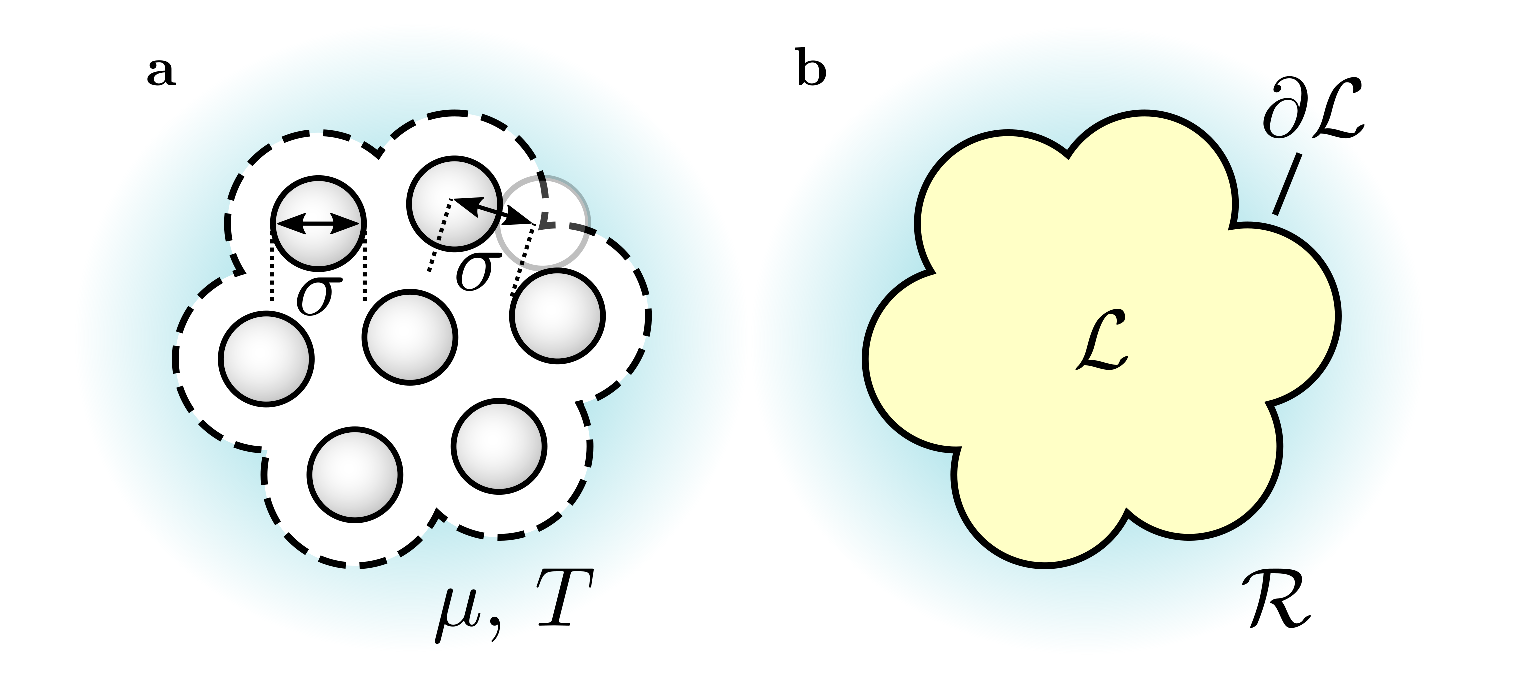
\includegraphics[width=\linewidth]{droplet-morph}
  \caption{
    The system considered showing
    (a) the local particles surrounded by the remaining liquid acting as a thermal reservoir at fixed chemical potential and temperature, and
    (b) partition of space into the local $\mathcal{L}$ and remaining $\mathcal{R}$ components with dividing surface $\partial\mathcal{L}$.
    In this work $\mathcal{L}$ is chosen as the space inaccessible to the centre of a test particle (shown faded) representing the remaining liquid.
  }
\end{SCfigure}

For systems with excluded volume interactions, we can divide the space into a local component $\mathcal{L} \subset \mathbb{R}^d$ of volume $V_\mathcal{L}$ inaccessible to solvent degrees of freedom and the remaining space $\mathcal{R} = \mathbb{R}^d \setminus \mathcal{L}$ of volume $V_\mathcal{R}$ filled by the rest of the liquid (Fig. \ref{fig:system}).
The total volume is $V_\mathcal{L} + V_\mathcal{R}$ so the homogeneous grand potential is
\begin{equation*}
  \Omega_{hom} = -p (V_\mathcal{L} + V_\mathcal{R}).
\end{equation*}
After inserting the inhomogeneity the total volume accessible to the rest of the liquid will be reduced by $V_\mathcal{L}$, so the grand potential becomes
\begin{equation*}
  \Omega = -p V_\mathcal{R} + \Omega_{ex}[\partial\mathcal{L}],
\end{equation*}
where $\Omega_{ex}$ is an excess term brought about by the introduction of a dividing surface $\partial\mathcal{L}$ between the two liquid components.
Subtracting these two expressions gives
\begin{equation*}
  \Delta \Omega = p V_\mathcal{L} + \Omega_{ex}[\partial\mathcal{L}].
\end{equation*}
This dividing surface has area $A_{\partial\mathcal{L}}$, creating a surface tension $\gamma$ so we can write the excess term as
\begin{equation*}
  \Omega_{ex}[\partial\mathcal{L}] =
  \gamma[\partial\mathcal{L}] A_{\partial\mathcal{L}}
\end{equation*}
which is a formal definition of surface tension for a choice of dividing surface.
We know from density functional theory that the excess free energy will be a functional of the inhomogeneous density profile, which will in turn depend on the shape of boundary; we write $\gamma = \gamma[\partial \mathcal{L}]$ to indicate this functional dependance on the surface shape.
The \emph{solvation form} of the inhomogeneous grand potential term in \eqref{eq:potential-mean-force} is then
\begin{equation}\label{eq:surface-tension}
  \Delta \Omega[\mathcal{L}] =
  p V_\mathcal{L} + \gamma[{\partial\mathcal{L}}] A_{\partial\mathcal{L}}.
\end{equation}
The problem of determining the $n$-particle distributions has been reduced to a solvation problem: we must find the surface tension between a solute (the specific local arrangement) and a solvent (the rest of the liquid).
We will use the solute--solvent language interchangeably with the local--bulk description.

Note that the surface tension is not unique as only the total grand potential must be independent of the choice of $\partial\mathcal{L}$ and can even change its sign for some choices of dividing surface \cite{Bryk2003}.
We will primarily focus on one-component liquids with particles of diameter $\sigma$.
We choose the \emph{solvent accessible surface} \cite{Lee1971} as the dividing surface such that $\mathcal{L} = \cup_{i=1}^n B^d_\sigma(\vec{r}_i)$ (Fig.\ \ref{fig:system}).

Before moving on, we will briefly comment on extensions of the results of this section.
First, it is straightforward to extend \eqref{eq:distribution-functions} and \eqref{eq:potential-mean-force} to mixtures; for an $m$-component mixture the potential of mean force is nearly identical
\begin{equation}
  \begin{split}
    \phi^{(\{n_i\})}(\vec{r}^n) &\equiv
    - k_B T \ln{g^{(n)}(\vec{r}^n)} \\
    &=
    U_n + \Delta\Omega - \sum_{i=1}^m n_i \mu_i^{ex},
  \end{split}
\end{equation}
where $\{n_i\}$ for $i = 1, \cdots, m$ is the number of each species of particle, and $\mu_i^{ex}$ is the excess chemical potential of species $i$.
Second, for more complicated interaction potentials (i.e.\ beyond pair potentials) the decomposition between internal interactions and grand potential breaks down; the internal structure of droplet the matters more\todo{rephrase this sentence}.
Finally, for soft potentials the definition of the potential of mean force is unaffected as we did not rely on particles being hard in its derivation, however the solvation expression will be affected.
For soft interactions it is impossible to define meaningful volumes which divide the local and bulk degrees of freedom: use of \eqref{eq:surface-tension} would be an approximation for soft potentials.
However, a plausible extension would be to replace the volume term by
\begin{equation}
  V_\mathcal{L} \to \int e^{-\beta \phi(\vec{r})} \, d\vec{r}
\end{equation}
where $\phi$ is the external potential caused by the inhomogeneity.
This reduces to the accessible volume as $\phi$ becomes a hard interaction.\todo{Can logarithmic surface tension corrections (capillary waves) destroy the formal result?}

\subsection{Grand potential is not an analytic function}

Here we demonstrate that the grand canonical cost of insertion contains singularities, so \emph{any} representation as an analytic function must necessarily be approximate.
This argument is a reformulation of those arguments made in the original scaled particle theories, as it was originally made for three-dimensional hard spheres by Reiss and coworkers in \cite{Reiss1959,Reiss1960,Mandell1976} discussed in detail in references
generalised to the noble gases \cite{Helfand1960}, hard disks \cite{Helfand1961}, mixtures \cite{Lebowitz1965} and more recently to hard sphere pairs in \cite{Stillinger2006,Chatterjee2006}.
Not sure: \cite{Reiss1961,Frisch1964,Reiss1965,Reiss1974,Tully-Smith1970,Harris1971}.

Discontinuity argument: probabilty that \emph{exactly} zero hard spheres contained in a spherical region of radius $R$ is \cite{Mandell1976}
\todo{I have lifted this wording almost exactly from Mandell \& Reiss, so rewrite this to avoid plagiarism}
\begin{equation}\label{eq:spt-zero-cavity-p}
  p_0(R) = 1 + \sum_{n=1}^{\infty} (-1)^n F^{(n)}(R)
\end{equation}
where $F^{(n)}(R)$ is the average number of $n$-tuples of hard spheres contained in the region defined via
\begin{equation}\label{eq:spt-tuple-function}
  F^{(n)} = \frac{\rho^n}{n!} \int_{\mathbb{V}_R} g^{(n)}(\vec{r}^n) \, d\vec{r}^n
\end{equation}
clearly $F^{(n)}(R) = 0$ for $R < R_n$, the minimum radius capable of containing the $n$ hard spheres.
At any given state point $g^{(n)}$ will be bounded from above by some finite number%
\marginfootnote{Typically we would expect this to occur where the maximum number of particles are in contact, however that is not a necessary assumption for this argument.},
so we can write the inequality
\begin{equation}\label{eq:spt-tuple-function-upper-bound}
  \begin{split}
    F^{(n)}(R) &\le
    \frac{\rho^n}{n!}
    \max_{\mathbb{R}^{dn}}{\left(g^{(n)}\right)}
    \int_{\mathbb{V}_R} \, d\vec{r}^n \\
    &=
    \frac{\rho^n}{n!}
    \max_{\mathbb{R}^{dn}}{\left(g^{(n)}\right)}
    (V_R)^n,
  \end{split}
\end{equation}
but because of the hard core interaction there will be heavy restrictions on allowable values of $n$ for any $R$.
Defining $R_n$ as the smallest $R$ such that $n$ particles can be accommodated, we expect
\begin{subequations}\label{eq:F-scaling}
  \begin{equation}
    F^{(n)}(R) =
    \begin{cases}
      0 & \quad R < R_n \\
      \mathcal{O}\left( \left(V_R\right)^n \right) & \quad R > R_n
    \end{cases}
  \end{equation}
\end{subequations}
where the latter polynomial is motivated by the same argument as used in \eqref{eq:spt-tuple-function-upper-bound}.
Noting that $V_R \propto R^d$ this can be expressed alternatively as a polynomial in $R$
\begin{subequations*}
  \begin{equation}
    F^{(n)}(R) =
    \begin{cases}
      0 & \quad R < R_n \\
      \mathcal{O}\left( R^{dn} \right) & \quad R > R_n
    \end{cases}
  \end{equation}
\end{subequations*}
Applying this bound to \eqref{eq:spt-zero-cavity-p} gives bounds on the scaling of $p_0$ as
\begin{equation}\label{eq:spt-p-scaling}
  p_0(R) =
  \mathcal{O}\left( R^{dn} \right)
  \quad R_n < R < R_{n+1}.
\end{equation}
From \eqref{eq:spt-p-scaling} we expect to see singular behaviour at the points $\{R_n\}$.
To look at this in detail we define
\begin{equation}
  p_0^{(n)}(R) = 1 + \sum_{m=1}^n (-1)^m F^{(m)}(R)
\end{equation}
such that $p_0 = p_0^{(n)}$ for $R \le R_{n+1}$.
Approaching the singular point $R_n$ we find the deviation from the solution for $R < R_n$ is thus
\begin{equation}
  \Delta p_0(R) \equiv
  p_0(R) - p_0^{(n-1)}(R) = (-1)^n F^{(n)}(R)
  \qquad R < R_{n+1}
\end{equation}
i.e.\ the singular behaviour is entirely contained in $F^{(n)}$.
Noting that polynomials of degree $n$ have vanishing $(n+1)$th derivatives, and $V_R \propto R^d$, we thus expect a discontinuity in the $(dn)$th derivative of $p_0$ about $R=R_n$.
Note that a discontinuity in the $dn$th derivative of $f(p_0(R))$ will be inherited from $p_0$ so long as $f$ is a suitably smooth function.
Thus $\Omega$ will feature a discontinuity in its $dn$th derivative about $R_n$, and $G$ in its $(dn+1)$th derivative.

Note that we have not quite proven that the singular behaviour actually occurs at any of the points $\{R_n\}$, because it is possible for the form of $g^{(n)}$ to eliminate singular behaviour.
We will eliminate this physically implausible scenario by showing that $F^{(n)}$ is bounded from below by $\mathcal{O}(R^{dn})$ so that it must take the form of this polynomial in the region $R > R_n$.
Then the argument above shows that singularities must occur in the indicated derivatives for hard spheres.

First, we note that for hard interactions the pair potential restricts the domain of integration in \eqref{eq:spt-tuple-function} to those configurations where particles do not overlap $\mathbb{V}_R'$, that is
\begin{equation}\label{eq:spt-tuple-integrand-lower-bound}
  \int_{\mathbb{V}_R} g^{(n)}(\vec{r}^n) d\vec{r}^n =
  \int_{\mathbb{V}_R'} y^{(n)}(\vec{r}^n) d\vec{r}^n \ge
  \min_{\mathbb{R}^{dn}}{\left(y^{(n)}(\vec{r}^n)\right)} V(\mathbb{V}_R')
\end{equation}
using the definition of the cavity function $y^{(n)}$ in \eqref{eq:cavity-functions}.
Note that in general $y^{(n)}(\vec{r}^n) > 0$, so as long as we just need to find some minimal set of configurations where $V(\mathbb{V}_R')$ is nonzero and scales as $\mathcal{O}(R^{dn})$ in order to complete the lower bound.
We consider a cavity of size $R=R_n$ where an arrangement%
\marginfootnote{It is possible that multiple arrangements become viable at the same radius, though this does not effect the substance of the argument.
  In this case the lower bound \eqref{eq:spt-tuple-function-lower-bound} will be multiplied by the degeneracy of $n$-particle packings at $R=R_n$, not affecting the scaling with $R$.}
of $n$ spheres becomes possible.
As this is the minimum radius required, the particles will be in contact.
If the cavity size $R$ is increased infinitesimally by an amount $\epsilon$, it is possible to affinely transform the particle positions
\begin{equation*}
  \vec{r}^{(n)} \to \left(1 + \frac{\epsilon}{2}\right) \vec{r}^{(n)}
\end{equation*}
so every particle can move up to $\epsilon/2$ in any direction without leaving the cavity or overlapping another sphere.
This gives us
\begin{equation*}
  V\left(\mathbb{V}_{R+\epsilon}'\right) \ge
  \left[ \omega_d \left(\frac{\epsilon}{2}\right)^d \right]^n
\end{equation*}
so from \eqref{eq:spt-tuple-function} and \eqref{eq:spt-tuple-integrand-lower-bound} we have
\begin{equation}\label{eq:spt-tuple-function-lower-bound}
  F^{(n)}(R_n+\epsilon) \ge
  \min_{\mathbb{R}^{dn}}{\left(y^{(n)}(\vec{r}^n)\right)}
  \, \left[ \omega_d \left(\frac{\epsilon}{2}\right)^d \right]^n \ge
  \mathcal{O}(\epsilon^{dn})
\end{equation}
where the right hand side is also a polynomial in $R$ so $F^{(n)}(R)$ is bounded from below by $\mathcal{O}(R^{dn})$.
Thus comparing the bounds \eqref{eq:spt-tuple-function-lower-bound} and \eqref{eq:spt-tuple-function-upper-bound} we see that
\begin{equation}
  \mathcal{O}(R^{dn}) \le F^{(n)}(R) \le \mathcal{O}(R^{dn})
  \quad R > R_n
\end{equation}
and so $F^{(n)}$ must scale as $R^{dn}$, thus completing the proof.

%A spherical cavity of radius $R=$ can accommodate the centres of 3 hard spheres
%Finding the arrangement of $n$ spheres which minimises its bounding sphere is a hard problem, but we can .

\begin{SCtable}
  \begin{minipage}[b]{\linewidth}
  \centering
  \begin{tabular}{ccc}
    \toprule
    $n$ & $R_n$ & Discontinuity \\
    \midrule
    \multicolumn{3}{c}{$d = 3$} \\
    \midrule
    1 & 0 & -- \\
    2 & $\frac{\sigma}{2}$ & $\Omega'', g'$ \\
    3 & $\frac{\sigma}{\sqrt{3}}$ &
    $\frac{\partial^6 \Omega}{\partial R^6}, \frac{\partial^5 g}{\partial R^5}$ \\
    4 & ${\sqrt{\frac{3}{8}}} \sigma$ &
    $\frac{\partial^9 \Omega}{\partial R^9}, \frac{\partial^8 g}{\partial R^8}$ \\
    \multicolumn{3}{c}{$d = 1$} \\
    \midrule
    1 & 0 & -- \\
    \midrule
    \multicolumn{3}{c}{$d = 2$} \\
    \midrule
    1 & 0 & -- \\
    \bottomrule
  \end{tabular}
  \end{minipage}
  \caption{Abc.}
\end{SCtable}

\subsection{Scaled particle theory}

\todo{Write down other exact sum rules that could be used.}
We describe here in more detail the derivation of the first set of morphometric coefficients, equivalent to those given in \cite{Hansen-Goos2006} through fundamental measure theory (FMT).
The derivation sketched below avoids use of FMT, instead favouring a geometric formulation equivalent to the scaled particle approach of Reiss \emph{et al}.\ \cite{Reiss1959,Reiss1960}.
The standard scaled particle approach considers an expansion of the grand potential surrounding a spherical solute in powers of radii; here, we modify the \emph{ansatz} to use morphological measures instead, so that the resulting theory is more naturally extended to geometries of arbitrary shapes.
Additionally, we impose the Carnahan-Starling equation of state as an \emph{input} whereas the Percus-Yevick equation of state is an \textit{output} of standard scaled particle approaches.

Following the protocol of scaled particle theories, we consider the insertion of a hard ball of radius $R-\frac{\sigma}{2}$ into the liquid at the origin.
This choice of radius ensures that contact with the \emph{center} of solvent particles occurs at distance $R$ from the point of insertion i.e.\ $\rho(r) = 0$ for $r < R$.
Writing the change in the grand potential due to the insertion of the ball in its morphometric form (from \eqref{eq:surface-tension} and \eqref{eq:morphometric-surface-tension} of the main text), we have the \emph{ansatz}
\begin{equation}\label{eq:morph-ball-solvation}
  \Delta \Omega(R) =
  \frac{4\pi R^3}{3} p +
  4\pi R^2 \, \gamma_\infty +
  4\pi R \, \kappa +
  4 \pi \, \overline{\kappa}.
\end{equation}
If an equation of state for the pressure is taken as input, only three equations are needed to set the remaining coefficients of surface tension $\gamma_\infty, \kappa$ and $\overline{\kappa}$.

Restating the expressions for the insertion of a hard point and a new particle from the main text as
\begin{align}
  \label{eq:spt-point} \Delta\Omega(R=0) &= -k_B T \ln{(1- \eta)}, \\
  \label{eq:spt-mu} \Delta\Omega\left(R=\frac{\sigma}{2}\right) &= \mu^{ex},
\end{align}
we need one more equation to set the thermodynamic coefficients for the theory.
Following Ref.\ \cite{Bryk2003} we take the normal derivative of $\Omega$ with respect to $R$, and noting that $\Delta\Omega(R) = \Omega(R) - \Omega_{hom}$ gives
\begin{equation}\label{eq:spt-derivative}
  \left( \frac{\partial \Delta \Omega}{\partial R} \right)_{\mu,V,T} =
  \left( \frac{\partial \Omega}{\partial R} \right)_{\mu,V,T} =
  \int
  \frac{\delta \Omega[\rho_0(\vec{r})]}{\delta \rho}
  \left( \frac{\partial \rho_0(\vec{r})}{\partial R} \right)_{\mu,V,T}
  \, d\vec{r} +
  \int
  \rho_0(\vec{r})
  \left( \frac{\partial \phi_{ext}(\vec{r})}{\partial R} \right)_{\mu,V,T}
  \, d\vec{r},
\end{equation}
where $\rho_0$ is the equilibrium density profile and $\phi_{ext}$ is the external potential (i.e.\ the potential of the ball).
In equilibrium $\Omega$ is minimised so
\begin{equation}
  \left.
  \frac{\delta \Omega[\rho(\vec{r}); \phi_{ext}]}{\delta \rho}
  \right|_{\rho(\vec{r})=\rho_0(\vec{r})} = 0,
\end{equation}
so the first integral in \eqref{eq:spt-derivative} vanishes.
As the ball is hard, the external potential and its derivative are zero everywhere except at the surface $R$ where both $\rho_0$ and $\phi_{ext}$ are discontinuous.
We consider its Boltzmann weight, i.e.\
\begin{equation}
  e^{-\beta\phi_{ext}(\vec{r})} = \Theta(|\vec{r}| - R).
\end{equation}
Taking the derivative of both sides gives
\begin{equation}
  \beta\left( \frac{\partial\phi_{ext}(\vec{r})}{\partial R} \right)_{\mu,V,T} =
  \delta(|\vec{r}| - R) e^{\beta\phi_{ext}(\vec{r})}
\end{equation}
Inserting this expression into \eqref{eq:spt-derivative} and using the fact that $\rho(\vec{r}) e^{\beta\phi_{ext}(\vec{r})}$ is continuous (c.f.\ Ref.\ \cite{Hansen2013}) gives the contact theorem
\begin{equation}
  \beta \left( \frac{\partial \Omega}{\partial R} \right)_{\mu,V,T} =
  4\pi R^2 \rho(R).
\end{equation}
When $R = \sigma$ the inserted ball is equivalent to the hard sphere particles themselves, so $\Omega = \mu^{ex}$ and the contact density is $\rho(\sigma) = \rho \, g^{(2)}(\sigma)$ giving
\begin{equation}\label{eq:spt-contact-density}
  \left. \beta \left( \frac{\partial \Delta \Omega}{\partial R} \right)_{\mu,V,T}
  \right|_{R = \sigma}
  =
  \left. \beta \left( \frac{\partial \Omega}{\partial R} \right)_{\mu,V,T}
  \right|_{R = \sigma}
  =
  %\beta \frac{\partial \mu^{ex}}{\partial \sigma} =
  4\pi \sigma^2 \rho \, g^{(2)}(\sigma),
\end{equation}
or written in morphometric form using \eqref{eq:morph-ball-solvation} we have
\begin{equation}
  4\pi \sigma^2 \, p +
  8\pi \sigma \, \gamma_\infty +
  4\pi \, \kappa =
  \frac{4\pi \sigma^2 \rho}{\beta} \, g^{(2)}(\sigma).
\end{equation}
Applying the virial theorem (equation \eqref{eq:contact-g} in the main text) to the right hand side gives the final expression:
\begin{equation}\label{eq:spt-virial}
  4\pi \sigma^2 \, p +
  8\pi \sigma \, \gamma_\infty +
  4\pi \, \kappa =
  \frac{6}{\beta\sigma} \left( \frac{\beta p}{\rho} - 1 \right).
\end{equation}
Together \eqref{eq:spt-point}, \eqref{eq:spt-mu} and \eqref{eq:spt-virial} form a complete system of equations which we solve to obtain the coefficients
\begin{subequations}
  \begin{align}
    \frac{\beta \gamma_\infty^{WBII}}{R \rho} &=
    \left(\frac{\pi}{6\eta^2} - \frac{5\pi}{18\eta}\right) p -
    \frac{\mu^{ex}[p]}{3\eta} -
    \frac{\ln{(1-\eta)}}{3\eta} -
    \frac{1}{\eta}
    \label{eq:spt-gamma}
    \\
    \frac{\beta \kappa^{WBII}}{R^2\rho} &=
    \left( \frac{4\pi}{9\eta} - \frac{\pi}{2\eta^2} \right) p +
    \frac{4\mu^{ex}[p]}{3\eta} + \frac{4\ln{(1-\eta)}}{3\eta} + \frac{3}{\eta}
    \\
    \frac{\beta \overline{\kappa}^{WBII}}{R^3\rho} &=
    \left( \frac{\pi}{3\eta^2} - \frac{2\pi}{9\eta} \right) p -
    \frac{\mu^{ex}[p]}{\eta} - \frac{4\ln{(1-\eta)}}{3\eta} - \frac{2}{\eta}.
  \end{align}
\end{subequations}
Inserting the Carnahan-Starling parameters \eqref{eq:cs-pressure} and \eqref{eq:cs-mu} gives the coefficients explicitly as
\begin{subequations}
  \begin{align}
    \frac{\beta p^{WBII}}{\rho} &=
    \frac{1 + \eta + \eta^2 - \eta^3}{(1-\eta)^3}
    \\
    \frac{\beta \gamma_\infty^{WBII}}{R\rho} &=
    -\frac{1 + 2\eta + 8\eta^2 - 5\eta^3}{3(1-\eta)^3}
    - \frac{\ln{(1-\eta)}}{3\eta}
    \\
    \frac{\beta \kappa^{WBII}}{R^2\rho} &=
    \frac{4 - 10\eta + 20\eta^2 - 8\eta^3}{3(1-\eta)^3} + \frac{4 \ln{(1-\eta)}}{3\eta}
    \\
    \frac{\beta \overline{\kappa}^{WBII}}{R^3\rho} &=
    - \frac{4 - 11\eta + 13\eta^2 - 4\eta^3}{3(1-\eta)^3} - \frac{4 \ln{(1-\eta)}}{3\eta},
  \end{align}
\end{subequations}
which are \emph{identical} to the coefficients derived from the WBII free energy functional in Ref.\ \cite{Hansen-Goos2006}.
Remarkably, we have obtained these coefficients through a route completely different from their original derivation.
In Ref.\ \cite{Hansen-Goos2006} the coefficients were determined within FMT by taking the limit of a binary mixture where one component is infinitely dilute.
Here we completely avoided FMT, in favour of geometrical arguments similar to standard scaled particle approaches.
This suggests that the above scaled particle argument is somehow built into the structure of the WBII functional; we note that this is a nonobvious fact which cannot be determined from the form of the functional alone, nor is it obvious how it emerges from its original derivation.

Finally, note that (as described in the main text) the resulting $g^{(2)}$ performs poorly in the supercooled regime as compared with the ``exact'' result from virial theorem i.e.\ Eq.\ \eqref{eq:contact-g} in the main text.
In Fig.\ \ref{fig:contact-g} we plot the contact value with this set of coefficients, finding that it is reasonably accurate until around the freezing density where contact correlations spuriously decay.
The next section will detail how to modify the derivation to produce coefficients which describe more accurate correlation functions at high densities.

\begin{SCfigure}[h]
 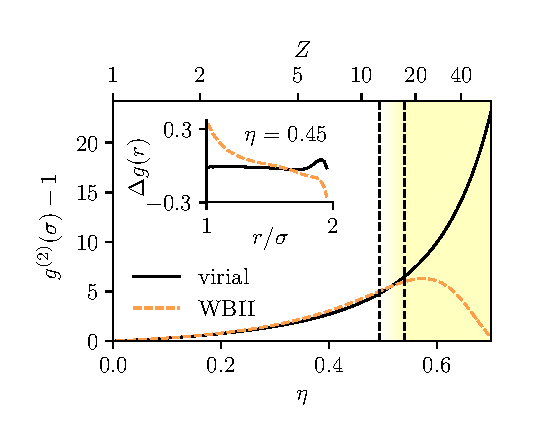
\includegraphics[width=\linewidth]{g2_contact}
 \caption{
   Contact values of the radial distribution function against volume fraction $\eta$ and reduced pressure $Z = \beta p / \rho$ for the hard sphere liquid using Eq.\ \eqref{eq:contact-g} from the main text with Eq. \eqref{eq:g2-explicit} for the explicit form of $g^{(2)}$, assuming the Carnahan-Starling equation of state.
   Contact values are determined with two sets of morphometric coefficients: WBII (section \ref{sec:spt-route} and Ref.\ \cite{Hansen-Goos2006}) which performs poorly in the supercooled regime, and coefficients derived in this work (section \ref{sec:virial-route}) using the virial theorem which is exact by construction.
   The hard sphere freezing and melting volume fractions are indicated by vertical dashed lines.
   Inset: the errors $\Delta g = g^{(2)} - g^{(2)}_{MD}$ where $g^{(2)}_{MD}$ is determined from molecular dynamics simulations (c.f.\ section \ref{SI:molecular-dynamics}), showing the new theory also improves the accuracy away from contact.
   %\todo{Remove the inset and make that its own figure.}
 }
\label{fig:contact-g}
\end{SCfigure}

\subsection{Aside: scaled particle theory extension for dimers}

I was unaware of work by Stillinger et al \cite{Stillinger2006} before publishing on the morphometric approach, but upon discovering this work I realised their ideas are very similar in nature.
Here I present similar results but using the morphometric notation.%
\todo{The purpose of this section needs to be fleshed out and made \emph{very} clear, otherwise the reader will get lost quickly.
  This section \emph{is} important as we explore the boundaries of where the morphometric approach can fail: this is a great testbed for continuity, and allows us to argue the accuracy of the approach applied to local structures.}

We have the probability of any number of particles existing inside the cavity
\begin{equation}
  \sum_{n=0}^\infty p_n (\lambda) = 1
\end{equation}
Giving the probability the cavity is empty due to a spontaneous thermal fluctuation
as
\begin{equation}
  p_0 (\lambda) = e^{-\beta W(\lambda)}
  = 1 - \sum_{n=1}^\infty p_n (\lambda).
\end{equation}
The singular nature of the hard sphere interaction ensures there is a maximum number of particles that can fit inside any finite sized cavity (the optimal packing), so we define
\begin{equation}
  n^*(\lambda) = \max{n(\lambda)},
\end{equation}
and thus
\begin{equation}
  p_0 (\lambda) = e^{-\beta W(\lambda)}
  = 1 - \sum_{n=1}^{n^*(\lambda)} p_n (\lambda).
\end{equation}

Following Stillinger we generalise to two cavities.
Define work to insert both cavities as $W^{(2)}(r,\lambda)$.
We then have the generalisaton
\begin{equation}
  p_0^{(2)} (\lambda) = e^{-\beta W^{(2)}(\lambda)}
  = 1 - \sum_{n=1}^{\max{n^{(2)}(\lambda)}} p_n^{(2)} (\lambda).
\end{equation}
We have the conditions:%
\todo{Make this notation more consistent and able to handle different numbers of cavities. We don't want to just recycle Stillinger's notation: we want to be consistent with the rest of the thesis.}
\begin{align}
  \lim_{r \to 0} W^{(2)}(r; \lambda) &= W^{(1)}(\lambda) \\
  \max{n^{(2)}(r; \lambda)} &= 1
  \quad \forall \; r + 2\lambda < 1 \\
  \lim_{r \to \infty} W^{(2)}(r; \lambda) &= 2 W^{(1)}(\lambda) \\
  \max{n^{(2)}(r; \lambda)} &\le 2 \max{n^{(1)}(\lambda)}
  \quad \forall \; r > 2\lambda
\end{align}
\todo{Need to define $\lambda$ as the cavity diameter}[4cm]
Which gives us the `point' insertion condition (where $\max{n^{(2)}(r; \lambda)} = 1$)
\begin{equation}
  \beta W^{(2)}(r; \lambda) = -\ln (1 - \rho V(r; \lambda))
\end{equation}

Hausdorff distance is simply $r$, so how the hell is the Euler characteristic of their union continuous with respect to $r$? It is discontinuous at $r = 2\lambda$.

\subsection{Morphometric approach}

Justification of assumptions: additivity, continuity and motion invariance.

\subsection{Virial route}

In this section we give the detailed steps used in the derivation of the new set of morphometric coefficients, following the direction laid out in the main text.
In section \ref{SI:two-particles} above the morphological form of $g^{(2)}$ was computed explicitly; this derivation imposes the contact density using $\rho(\sigma) = \rho \, g^{(2)}(\sigma)$ with this explicit form.

From \eqref{eq:g2-explicit} the potential of mean force for neighbouring particles reduces to $\phi^{(2)}(r) = \Delta\Omega(r) - 2\mu^{ex}$ if they do not overlap, giving
\begin{equation}
  \begin{split}
  \phi^{(2)}(r) &\equiv - k_B T \ln g^{(2)}(r) \\
  &= pV(r) + \gamma_\infty A(r) + \kappa C(r) + \overline{\kappa} X(r) - 2\mu^{ex}
  \quad \forall \; \sigma \le r \le 2\sigma.
  \end{split}
\end{equation}
Inserting the morphological quantities at contact from \eqref{eq:g2-explicit-morph} gives
\begin{equation}
  \phi^{(2)}(\sigma) =
  \frac{9\pi \sigma^3}{4} p +
  6\pi\sigma^2 \, \gamma_\infty +
  \left( 6\pi\sigma - \frac{\pi^2\sigma}{2\sqrt{3}} \right) \, \kappa +
  4\pi \, \overline{\kappa}
  - 2\mu^{ex}[p].
\end{equation}
Equating this with $-k_B T \ln g^{(2)}(\sigma)$ and using the virial theorem (Eq.\ \eqref{eq:contact-g} in the main text) gives the final expression
\begin{equation}\label{eq:v-virial}
  \frac{9\pi \sigma^3}{4} p +
  6\pi\sigma^2 \, \gamma_\infty +
  \left( 6\pi\sigma - \frac{\pi^2\sigma}{2\sqrt{3}} \right) \, \kappa +
  4\pi \, \overline{\kappa} =
  2\mu^{ex}[p] - \beta^{-1} \ln{\frac{3}{2\pi \rho \sigma^3} \left( \frac{\beta p}{\rho} - 1 \right)}.
\end{equation}
We will use this last expression instead of the contact theorem \eqref{eq:spt-virial} in order to obtain new coefficients.
Together \eqref{eq:spt-point}, \eqref{eq:spt-mu} and \eqref{eq:v-virial} solve to give coefficients:
\begin{subequations}
  \begin{align}
    \frac{\beta \gamma_\infty^{V}}{R\rho} &=
    \frac{ (18\pi - 7\sqrt{3} \pi^2) p + 6\sqrt{3}\pi \mu^{ex}[p]
      - 6(12 - \sqrt{3}\pi) \ln{(1-\eta)}
      - 72\ln{\left( \frac{\pi p - 6\eta}{24\eta^2} \right)} }
    {54(\sqrt{3}\pi - 4) \eta}
    \label{eq:virial-gamma}
    \\
    \frac{\beta \kappa^{V}}{R^2\rho} &=
    \frac{ 5\pi p - 12 \mu^{ex}[p] + 24 \ln{(1-\eta)}
      + 36\ln{\left( \frac{\pi p - 6\eta}{24\eta^2} \right)} }
    {9(\sqrt{3}\pi - 4) \eta}
    \\
    \frac{\beta \overline{\kappa}^{V}}{R^3\rho} &=
    - \frac{
      (18\pi - 2\sqrt{3} \pi^2) p - (36 - 3\sqrt{3}\pi) \mu^{ex}[p] + 12\sqrt{3}\pi \ln{(1-\eta)}
      + 72\ln{\left( \frac{\pi p - 6\eta}{24\eta^2} \right)} }
    {27(\sqrt{3}\pi - 4) \eta},
  \end{align}
\end{subequations}
which upon insertion of the Carnahan-Starling parameters \eqref{eq:cs-pressure} and \eqref{eq:cs-mu} gives the coefficients explicitly as
\begin{subequations}
  \begin{align}
    \frac{\beta p^{V}}{\rho} &=
    \frac{1 + \eta + \eta^2 - \eta^3}{(1-\eta)^3} \\
    \frac{\beta \gamma_\infty^{V}}{R\rho} &=
    \frac{ 18\eta \frac{1 + \eta + \eta^2 - \eta^3}{(1-\eta)^3}
      + \sqrt{3}\pi\eta \frac{1 - 16\eta - 4\eta^2 + 7\eta^3}{(1-\eta)^3}
      - (12 - \sqrt{3}\pi) \ln{(1-\eta)}
      - 12\ln{\left( \frac{2 - \eta}{2(1-\eta)^3} \right)} }
    {9(\sqrt{3}\pi - 4) \eta} \\
    \frac{\beta \kappa^{V}}{R^2\rho} &= -
    \frac{ 2\eta \frac{11 - 23\eta + \eta^2 + 5\eta^3}{(1-\eta)^3}
      - 8 \ln{(1-\eta)}
      - 12\ln{\left( \frac{2 - \eta}{2(1-\eta)^3} \right)} }
    {3(\sqrt{3}\pi - 4) \eta} \\
    \frac{\beta \overline{\kappa}^{V}}{R^3\rho} &=
    \frac{ 12\eta \frac{5 - 12\eta + 3\eta^3}{(1-\eta)^3}
      - \sqrt{3}\pi\eta \frac{4 - 13\eta - \eta^2 + 4\eta^3}{(1-\eta)^3}
      - 4\sqrt{3}\pi \ln{(1-\eta)}
      - 24\ln{\left( \frac{2 - \eta}{2(1-\eta)^3} \right)} }
    {9(\sqrt{3}\pi - 4) \eta}.
  \end{align}
\end{subequations}
Unlike the WBII coefficients above these are entirely new, and produce significantly more accurate correlation functions at high densities as described in the main text.
The pair correlation produced by these coefficients (black line in Fig.\ \ref{fig:contact-g}) is self-consistent with CS at contact by construction, but as an additional bonus we find that the new coefficients provide a theory that outperforms the older WBII approach across the whole range of distances typical of neighbouring particles (inset of Fig.\ \ref{fig:contact-g}).
The latter observation enables us to accurately model complex many-particle local structures.

However, it should be noted that the planar surface tension $\gamma_\infty^{V}$ is considerably less accurate than $\gamma_\infty^{WBII}$ as compared with molecular dynamics studies in \cite{Davidchack2016}.
For this reason, WBII coefficients may give more accurate grand potentials (and thus correlations) for large solutes where the surface becomes approximately planar.

\section{Bulk virial approach}

\subsection{Outline}

As far as I know this is an original calculation, however it should be emphasised that this is merely an application of ideas from FMT to the (simpler) uniform system.
\todo{Emphasise that the resulting equations of state should be bad for anisotropic particles: it won't find any liquid crystalline transitions, and we expect multiple intersections to be a general rule for highly anistropic particles.}
My aim here is to introduce the ideas of FMT gradually in order to emphasise the role played by integral geometry.

Note that in mean field $d \gg 1$ it is argued that the dominant contributions come from the ring diagrams, i.e.\
\begin{equation*}
  \lim_{d \to \infty}
  \frac{\beta F_{ex}}{N} =
  \rho^2 \mayerdiagram{2} +
  \rho^3 \mayerdiagram{3} +
  \rho^4 \mayerdiagram[|.||.|]{4} +
  \rho^5 \, \mayerdiagram[|..||..|.|]{5} +
  \mathcal{O}(\rho^6)
\end{equation*}
whereas the contributing diagrams in for $d=1$ are the fully connected Ree-Hoover diagrams, i.e.\
\begin{equation*}
  \begin{aligned}
    \lim_{d \to 1}
    \frac{\beta F_{ex}}{N} &=
    \rho^2 \mayerdiagram{2} +
    \rho^3 \mayerdiagram{3} +
    \rho^4 \mayerdiagram{4} +
    \rho^5 \, \mayerdiagram{5} +
    \mathcal{O}(\rho^6) \\
    &=
    \rho^2 \fmtdiagram{2} +
    \rho^3 \fmtdiagram{3} +
    \rho^4 \fmtdiagram{4} +
    \rho^5 \fmtdiagram{5} +
    \mathcal{O}(\rho^6)
  \end{aligned}
\end{equation*}

\subsection{Exact result in one dimensions: hard rods}

Spheres in one dimensions are just line segments%
\marginfootnote{In fact, line segments are the only possible convex shape in one dimensions so hard rods are the one dimensional starting point for arbitrary (convex) shapes in higher dimensions.},
or rods, so one dimensional hard spheres are conventionally called hard rods.
The hard rod system is sufficiently simple that all of its equilibrium properties can be determined exactly, so it provides a good starting point for theories in higher dimensions.
Here we show how integral geometry can be used to determine the exact free energy (and thus the equation of state) for the hard rod system; this suggests approximations in higher dimensions to be discussed in the next section.

\begin{tcolorbox}[title=Multiple intersections of hard rods]
  Where every pairwise combination of $n$ rods overlap, there must be a region where all of them intersect, i.e.\
  \begin{equation}
    \prod_{i \le j} \mu_0(B_i \cap B_j) =
    \mu_0(\cap_{i=1}^n B_i)
  \end{equation}
  \emph{Proof:} Consider three rods whose centers are placed at $x_1, x_2, x_3$.
  Each rod overlaps so we have
  \begin{subequations}
    \begin{align}
      |x_2 - x_1| &\le \sigma \\
      |x_3 - x_1| &\le \sigma \\
      |x_3 - x_2| &\le \sigma
    \end{align}
  \end{subequations}
  The region of overlap between the first two particles is
  \begin{equation*}
    B_1 \cap B_2 =
    [\max{(x_1,x_2)} - \sigma, \min{(x_1,x_2)} + \sigma].
  \end{equation*}
  which implies
  \begin{equation}
    \max{(x_1,x_2)} - \sigma \le x_3 \le \min{(x_1,x_2)} + \sigma
  \end{equation}
  or $x_3 \in (B_1 \cap B_2)$.
\end{tcolorbox}

\begin{SCfigure}[H]
  \missingfigure[figwidth=\linewidth]{}
  \caption{If each pair of three hard rods overlap then this implies a region where all three mutually intersect.}
\end{SCfigure}

Therefore the diagram for the third virial coefficient becomes
\begin{equation}\label{eq:third-virial-diagram-replacement-1d}
  \mayerdiagram{3} = \fmtdiagram{3}
\end{equation}
where the latter \emph{intersection} diagram denotes an integral of the form
\begin{equation}
  \fmtdiagram{3} =
  \int_{\mathbb{E}_d^3}
  \mu_0 (g_1 B^d \cap g_2 B^d \cap g_3 B^d)
  \, dg_1 dg_2 dg_3.
\end{equation}
The result of \eqref{eq:third-virial-diagram-replacement-1d} generalises straightforwardly to the other fully connected diagrams.
For example, the fourth and fifth terms in the virial series are replaced by
\begin{align*}
  \mayerdiagram{4} &= \fmtdiagram{4} =
  \int_{\mathbb{E}^4}
  \mu_0 (\cap_{i=1}^4 g_i B^1)
  \, dg^4
  \\
  \mayerdiagram{5} &= \fmtdiagram{5} =
  \int_{\mathbb{E}^5}
  \mu_0 (\cap_{i=1}^5 g_i B^1)
  \, dg^5,
\end{align*}
and in general the $n$th fully connected diagram can be replaced by the integral
\begin{equation}
  \int_{\mathbb{E}_d^n}
  \mu_0 (\cap_{i=1}^n g_i B^1)
  \, dg^n \equiv \Gamma_n,
\end{equation}
without approximation.

We can do much better in $d=1$, for hard rods.
We have the pressure defined by
\begin{equation}
  \frac{\beta p}{\rho} =
  1 + \sum_{n=2}^\infty c_n (n-1) \rho^{n-1} \Gamma_n
\end{equation}
with $c_n = 1/n(n-1)$ \todo{I think you can get $c_n$ from the $d=0$ case: check this} giving
\begin{equation}
  \Gamma_n = \int_{\mathbb{E}_d^n} \mu_0 (B^d \cap_{i=2}^n g_i B^d) \, d^n g
\end{equation}
For $d=1$ we have
\begin{equation}
  \int_{\mathbb{E}} \mu_k (A \cap g B^1) \, dg =
  \begin{cases}
    \mu_0(A) \mu_1(B^1) + \mu_1(A) & \qquad k=0 \\
    \mu_1(A) \mu_1(B^1) & \qquad k=1
  \end{cases}
\end{equation}
which gives
\begin{equation}
  \begin{split}
    \Gamma_n &= \int_{\mathbb{E}^{n-1}} \Big(
    \mu_0 \left( B^1 \cap_{i=2}^{n-1} g_i B^1 \right)
    \mu_1(B^1) +
    \mu_1 \left( B^1 \cap_{i=2}^{n-1} g_i B^1 \right)
    \Big) \, d^{n-1} g \\
    &=
    \Gamma_{n-1} \mu_1(B^1) +
    \mu_1(B^1)^{n-1}.
  \end{split}
\end{equation}
Applying this formula iteratively gives
\begin{equation}
  \Gamma_n = n \mu_1(B^1)^{n-1}.
\end{equation}
\begin{equation}
  \frac{\beta p}{\rho} =
  1 + \sum_{n=2}^\infty \rho^{n-1} \mu_1(B^1)^{n-1}
\end{equation}
But $\rho = \eta / \mu_1(B^1)$ so we have
\begin{equation}
  \frac{\beta p}{\rho} =
  1 + \sum_{n=2}^\infty \eta^{n-1} =
  \sum_{n=0}^\infty \eta^{n} = \frac{1}{1 - \eta}
\end{equation}
which is convergent for all $|\eta| < 1$ although only positive volume fractions i.e.\ in the range $\eta \in [0,1]$ have any physical meaning.

\subsection{Approximate extension to $d > 1$ dimensions}

We make the replacement
\begin{equation}\label{eq:third-virial-diagram-replacement-general}
  \mayerdiagram{3} \approx \fmtdiagram{3}
\end{equation}
which is now approximate as can be seen from the counter example in Figure \ref{fig:lost-cases}.

\begin{SCfigure}[H]
  \missingfigure[figwidth=\linewidth]{}
  \caption{Lost cases of FMT.}
  \label{fig:lost-cases}
\end{SCfigure}

Simple example: Mayer-f two balls:
\begin{equation}
  \frac{\beta p}{\rho} - 1 =
  - \sum_{i=1}^\infty \frac{i}{i+1} \beta_i \rho^i =
  \frac{\rho}{2} \int_{\mathbb{E}_d} \mu_0 (B_d \cap g B_d) \, dg
  + \mathcal{O}(\rho^2)
\end{equation}
Volume fraction $\eta = \rho \omega_d$
\begin{equation}
  \frac{\beta p}{\rho} - 1 =
  \frac{\eta}{2 \omega_d}
  \int_{\mathbb{E}_d} \mu_0 (B_d \cap g B_d) \, dg
  + \mathcal{O}(\eta^2)
\end{equation}
For $d = 3$ this gives $4\eta + \mathcal{O}(\eta^2)$.
\begin{align*}
  \frac{\eta}{2 \omega_d}
  \int_{\mathbb{E}_d} \mu_0 (B_d \cap g B_d) \, dg &=
  \sum_{i=0}^{d}
  {d \brack i}^{-1}
  \mu_i(B_d) \mu_{d-i}(B_d) \\
  &=
  \frac{\eta}{2 \omega_d}
  \sum_{i=0}^{d}
  {d \brack i}^{-1}
  {d \brack i} \omega_i
  {d \brack d-i} \omega_{d-i} \\
  &=
  \frac{\eta}{2 \omega_d}
  \sum_{i=0}^{d}
  {d \brack i} \omega_i \omega_{d-i} \\
  &=
  \begin{cases}
    \frac{\eta}{2 \omega_2}
    (2 \omega_0 \omega_2 + \frac{\pi}{2} \omega_1^2)
    & \qquad d=2 \\
    \frac{\eta}{\omega_3}
    (\omega_0 \omega_3 + 2 \omega_1 \omega_2)
    & \qquad d=3
  \end{cases} \\
  &=
  \begin{cases}
    2 \eta & \qquad d=2 \\
    4 \eta & \qquad d=3
  \end{cases}
\end{align*}
using \eqref{eq:flag-coefficients-symmetry} and \eqref{eq:intrinsic-volume-ball-flag}.
\begin{equation*}
\end{equation*}

Ree-Hoover diagrams.
From the relation:
\begin{equation*}
  1 = e_{ij} - f_{ij}
\end{equation*}
we have the graphical representation of this rule as
\begin{equation*}
  \mayerdiagram[.]{2} =
  \mayerdiagram[:]{2} -
  \mayerdiagram[|]{2}
\end{equation*}
so
\begin{equation*}
  \begin{aligned}
    \mayerdiagram[|.||.|]{4} &=
    \mayerdiagram[|.||:|]{4} -
    \mayerdiagram[|.||||]{4} \\
    &=
    \mayerdiagram[|:||:|]{4} +
    \mayerdiagram[||||||]{4} -
    \mayerdiagram[|:||||]{4} -
    \mayerdiagram[||||:|]{4} \\
    &=
    \mayerdiagram[|:||:|]{4} +
    \mayerdiagram[||||||]{4} -
    2 \mayerdiagram[|:||||]{4}
  \end{aligned}
\end{equation*}
after using permutation invariance in the final step.
We will extend this by considering only the fully connected Ree-Hoover diagrams, as in
\begin{equation}
  \frac{\beta F^{ex}}{N} \approx
  \rho^2 \mayerdiagram{2} +
  \rho^3 \mayerdiagram{3} +
  \rho^4 \mayerdiagram{4} +
  \rho^5 \mayerdiagram{5}
  + \mathcal{O}(\rho^6)
\end{equation}
and then approximate these by considering only the subset of $n$-particle intersections as in
\begin{equation}
  \frac{\beta F^{ex}}{N} \approx
  \rho^2 \fmtdiagram{2} +
  \rho^3 \fmtdiagram{3} +
  \rho^4 \fmtdiagram{4} +
  \rho^5 \fmtdiagram{5}
  + \mathcal{O}(\rho^6)
\end{equation}

Defining the more general integral
\begin{equation}
  \Gamma_n^{(k)} = \int_{\mathbb{E}_d^n} \mu_k (B^d \cap_{i=2}^n g_i B^d) \, d^n g
\end{equation}
For $d=3$ we have
\begin{equation}
  \int_{\mathbb{E}} \mu_k (A \cap g B^3) \, dg =
  \begin{cases}
    \omega_3 \mu_0(A) + \omega_2 \mu_1(A) +
    \omega_1 \mu_2(A) + \omega_0 \mu_3(A)
    & \qquad k=0 \\
    \omega_3 \mu_1(A) + \frac{\pi}{2} \omega_2 \mu_2(A)
    + 2 \omega_1 \mu_3(A)
    & \qquad k=1 \\
    \omega_3 \mu_2(A) + 2 \omega_2 \mu_3(A) & \qquad k=2 \\
    \omega_3 \mu_3(A) & \qquad k=3
  \end{cases}
\end{equation}
so the lowest-order integrals for $n=2$ evaluate to
\begin{align}
  \Gamma_2^{(0)} &= 2 \omega_0 \omega_3 + 4 \omega_1 \omega_2 \\
  \Gamma_2^{(1)} &= 4 \omega_1 \omega_3 + \pi \omega_2^2 \\
  \Gamma_2^{(2)} &= 4 \omega_2 \omega_3 \\
  \Gamma_2^{(3)} &= \omega_3^2.
\end{align}
Iterating the integrals gives (evaluated in order of simplicity)
\begin{align}
  \Gamma_n^{(3)} &=
  \omega_3 \Gamma_{n-1}^{(3)}
  = \omega_3^n \\
  \Gamma_n^{(2)} &=
  \omega_3 \Gamma_{n-1}^{(2)} + 2 \omega_2 \Gamma_{n-1}^{(3)}
  \nonumber \\ &=
  \omega_3 \Gamma_{n-1}^{(2)} + 2 \omega_2 \omega_3^{n-1}
  = 2 n \omega_2 \omega_3^{n-1} \\
  \Gamma_n^{(1)} &=
  \omega_3 \Gamma_{n-1}^{(1)} +
  \frac{\pi}{2} \omega_2 \Gamma_{n-1}^{(2)} +
  2 \omega_1 \Gamma_{n-1}^{(3)}
  \nonumber \\ &=
  \omega_3 \Gamma_{n-1}^{(1)} +
  (n-1) \pi \omega_2^2 \omega_3^{n-2} +
  2 \omega_1 \omega_3^{n-1}
  \nonumber \\ &=
  \frac{n(n-1)}{2} \pi \omega_2^2 \omega_3^{n-2} +
  2n \omega_1 \omega_3^{n-1}
  \\
  \Gamma_n^{(0)} &=
  \omega_3 \Gamma_{n-1}^{(0)} +
  \omega_2 \Gamma_{n-1}^{(1)} +
  \omega_1 \Gamma_{n-1}^{(2)} +
  \omega_0 \Gamma_{n-1}^{(3)}
  \nonumber \\ &=
  \omega_3 \Gamma_{n-1}^{(0)} +
  \frac{(n-1)(n-2)}{2} \pi \omega_2^3 \omega_3^{n-3} +
  2(n-1) \omega_1 \omega_2 \omega_3^{n-2} +
  \nonumber \\ & \quad
  2(n-1) \omega_1 \omega_2 \omega_3^{n-2} +
  \omega_0 \omega_3^{n-1}
  \nonumber \\ &=
  \frac{n(n-1)(n-2))}{6} \pi \omega_2^3 \omega_3^{n-3} +
  2 n(n-1) \omega_1 \omega_2 \omega_3^{n-2} +
  n \omega_0 \omega_3^{n-1}
\end{align}
This gives
\begin{equation}
  \begin{split}
    \frac{\beta p}{\rho} &=
    1 + \sum_{n=2}^\infty \frac{1}{n} \frac{\eta^{n-1}}{\omega_3^{n-1}} \Gamma_n
    =
    1 + \sum_{n=1}^\infty \frac{1}{n+1} \frac{\eta^n}{\omega_3^n} \Gamma_{n+1}
    \\ &=
    1 + \sum_{n=1}^\infty \frac{1}{n+1} \frac{\eta^n}{\omega_3^n}
    \left(
    \frac{n(n-1)(n+1))}{6} \pi \omega_2^3 \omega_3^{n-2} +
    2 n(n+1) \omega_1 \omega_2 \omega_3^{n-1} +
    (n+1) \omega_0 \omega_3^{n}
    \right)
    \\ &=
    1 + \sum_{n=1}^\infty \eta^n
    \left(
    \frac{n(n-1)}{6} \pi \frac{\omega_2^3}{\omega_3^2} +
    2 n \frac{\omega_1 \omega_2}{\omega_3} +
    \omega_0
    \right)
    \\ &=
    \pi \frac{\omega_2^3}{6\omega_3^2}
    \sum_{n=0}^\infty
    n(n-1) \eta^n
    +
    2 \frac{\omega_1 \omega_2}{\omega_3}
    \sum_{n=0}^\infty n \eta^n
    +
    \left( 1 + \omega_0 \sum_{n=1}^\infty \eta^n \right)
    \\ &=
    \pi \frac{\omega_2^3}{6\omega_3^2}
    \eta^2
    \sum_{n=0}^\infty
    n(n-1) \eta^{n-2}
    +
    2 \frac{\omega_1 \omega_2}{\omega_3}
    \eta
    \sum_{n=0}^\infty n \eta^{n-1}
    +
    \sum_{n=0}^\infty \eta^n
    \\ &=
    \pi \frac{\omega_2^3}{6\omega_3^2}
    \eta^2
    \frac{2}{(1-\eta)^3}
    +
    2 \frac{\omega_1 \omega_2}{\omega_3}
    \eta
    \frac{1}{(1-\eta)^2}
    +
    \frac{1}{1-\eta}
    \\ &=
    \pi \frac{\pi^3}{6 (16 \pi^2 / 9)}
    \eta^2
    \frac{2}{(1-\eta)^3}
    +
    2 \frac{2 \pi}{4 \pi / 3}
    \eta
    \frac{1}{(1-\eta)^2}
    +
    \frac{1}{1-\eta}
    \\ &=
    \frac{3 \pi^2}{16}
    \eta^2
    \frac{1}{(1-\eta)^3}
    +
    3
    \eta
    \frac{1}{(1-\eta)^2}
    +
    \frac{1}{1-\eta}
    \\ &=
    \frac{A\eta^2}{(1-\eta)^3}
    +
    \frac{3\eta (1-\eta)}{(1-\eta)^3}
    +
    \frac{(1-\eta)^2}{(1-\eta)^3}
    \\ &=
    \frac{A \eta^2
    +
    3\eta - 3\eta^2
    +
    1-2\eta + \eta^2}{(1-\eta)^3}
    \\ &=
    \frac{1 + \eta + (A - 2) \eta^2}{(1-\eta)^3}
  \end{split}
\end{equation}
\begin{align*}
  A = 3 &= \frac{3\pi^2}{16} + B \\
  B &= 3\left( 1 - \frac{\pi^2}{16} \right) \\
  B &= \frac{48 - 3\pi^2}{16} \\
  B &= 3 - \frac{\pi \omega_2^2}{\omega_3^2} \\
\end{align*}
For $d=2$ we have
\begin{equation}
  \int_{\mathbb{E}} \mu_k (A \cap g B^2) \, dg =
  \begin{cases}
    \omega_2 \mu_0(A) + \omega_1 \mu_1(A) + \omega_0 \mu_2(A) & \qquad k=0 \\
    \omega_2 \mu_1(A) + \frac{\pi}{2} \omega_1 \mu_2(A) & \qquad k=1 \\
    \omega_2 \mu_2(A) & \qquad k=2
  \end{cases}
\end{equation}
so the lowest-order integrals for $n=2$ evaluate to
\begin{align}
  \Gamma_2^{(0)} &= 2 \omega_0 \omega_2 + \omega_1^2 \\
  \Gamma_2^{(1)} &= \pi \omega_1 \omega_2 \\
  \Gamma_2^{(2)} &= \omega_2^2.
\end{align}
Iterating the integrals gives (evaluated in order of simplicity)
\begin{align}
  \Gamma_n^{(2)} &=
  \omega_2 \Gamma_{n-1}^{(2)}
  = \omega_2^n \\
  \Gamma_n^{(1)} &=
  \omega_2 \Gamma_{n-1}^{(1)}
  + \frac{\pi}{2} \omega_1 \Gamma_{n-1}^{(2)}
  \nonumber \\ &=
  \omega_2 \Gamma_{n-1}^{(1)}
  + \frac{\pi}{2} \omega_1 \omega_2^{n-1}
  = \frac{n \pi}{2} \omega_1 \omega_2^{n-1} \\
  \Gamma_n^{(0)} &=
  \omega_2 \Gamma_{n-1}^{(0)}
  + \omega_1 \Gamma_{n-1}^{(1)}
  + \omega_0 \Gamma_{n-1}^{(2)}
  \nonumber \\ &=
  \omega_2 \Gamma_{n-1}^{(0)}
  + \frac{(n-1) \pi}{2} \omega_1^2 \omega_2^{n-2}
  + \omega_0 \omega_2^{n-1}
  \nonumber \\ &=
  \sum_{m=1}^n \omega_2^{n-m} \left(
  \frac{(m-1)\pi}{2} \omega_1^2 \omega_2^{m-2}
  + \omega_0 \omega_2^{m-1}
  \right)
  \nonumber \\ &=
  \omega_2^{n-2}
  \sum_{m=1}^n \left(
  \frac{(m-1)\pi}{2} \omega_1^2
  + \omega_0 \omega_2
  \right)
  \nonumber \\ &=
  \omega_2^{n-2}
  \left(
  \frac{n(n-1)\pi}{4} \omega_1^2
  + n \omega_0 \omega_2
  \right)
\end{align}
This gives
\begin{equation}
  \begin{split}
    \frac{\beta p}{\rho} &=
    1 + \sum_{n=2}^\infty \frac{1}{n} \frac{\eta^{n-1}}{\omega_2^{n-1}} \Gamma_n
    \\ &=
    1 + \sum_{n=1}^\infty \frac{1}{n+1} \frac{\eta^n}{\omega_2^n} \Gamma_{n+1}
    \\ &=
    1 + \sum_{n=1}^\infty \frac{1}{n+1} \frac{\eta^n}{\omega_2^n}
    \omega_2^{n-1}
    \left(
    \frac{n(n+1)\pi}{4} \omega_1^2
    + (n+1) \omega_0 \omega_2
    \right)
    \\ &=
    1 + \sum_{n=1}^\infty \eta^n
    \left(
    \frac{n\pi}{4} \frac{\omega_1^2}{\omega_2}
    + \omega_0
    \right)
    \\ &=
    1 + \sum_{n=1}^\infty (n+1) \eta^n =
    \sum_{n=0}^\infty n \eta^{n-1}
    = \frac{1}{(1-\eta)^2}
  \end{split}
\end{equation}
which is absolutely convergent for all $|\eta| < 1$, although only values in the range $\eta \in [0,1]$ have any physical meaning.

\subsection{Fundamental measure theory (FMT)}

\subsection{Many-body correlations from fundamental measure theory}

\begin{itemize}
\item $d+1$ weight functions
\item Exact decomposition of Mayer-f bond
\end{itemize}

We have 4 scalar weight functions
\begin{subequations}
  \begin{align}
    \omega_3^i(\vec{r}) &= \Theta(R_i - r), \\
    \omega_2^i(\vec{r}) &= \delta(R_i - r), \\
    \omega_1^i(\vec{r}) &= \frac{\omega_2^i(\vec{r})}{4\pi R_i}, \\
    \omega_0^i(\vec{r}) &= \frac{\omega_2^i(\vec{r})}{4\pi R_i^2},
  \end{align}
\end{subequations}
and 2 vector weight functions
\begin{subequations}
  \begin{align}
    \vec{\omega}_2^i(\vec{r}) &=
    \frac{\vec{r}}{r} \delta(R_i - r), \\
    \vec{\omega}_1^i(\vec{r}) &=
    \frac{\vec{\omega}_1^i(\vec{r})}{4\pi R_i}.
  \end{align}
\end{subequations}

Fourier transforming weight functions:
\begin{equation}
  \widetilde{\omega}_\alpha(\vec{k}) =
  \int \omega_\alpha (\vec{r}) e^{-i \vec{k}\cdot\vec{r}} \, d\vec{r}
\end{equation}
%% \begin{align}
%%   \widetilde{\omega}_3(\vec{k}) &=
%%   4\pi \frac{\sin{kR} - kR\cos{kR}}{k^3} \\
%%   \widetilde{\omega}_2(\vec{k}) &=
%%   4\pi R^2 \frac{\sin{kR}}{kR} \\
%%   \widetilde{\vec{\omega}}_2(\vec{k}) &=
%%   - i \vec{k} \widetilde{\omega}_3(\vec{k})
%% \end{align}
\begin{equation}
  \begin{aligned}
    c_{22}(\vec{r} = \vec{r}_2 - \vec{r}_1) &=
    \frac{1}{(2\pi)^3}
    \iint
    e^{-i (\vec{k}_1\cdot\vec{r}_1 + \vec{k}_2\cdot\vec{r}_2)}
    \widetilde{\omega}_2(\vec{k}_1)
    \widetilde{\omega}_2(\vec{k}_2)
    \delta{(\vec{k}_1 + \vec{k}_2)}
    \, d\vec{k}_1 d\vec{k}_2 \\
    &=
    \frac{1}{(2\pi)^3}
    \int
    e^{i \vec{k}_1 \cdot (\vec{r}_2 - \vec{r}_1)}
    \widetilde{\omega}_2(\vec{k}_1)
    \widetilde{\omega}_2(-\vec{k}_1)
    \, d\vec{k}_1 \\
    &=
    \frac{1}{(2\pi)^3}
    \int
    e^{i \vec{k} \cdot \vec{r}}
    \widetilde{\omega}_2(\vec{k})^2
    \, d\vec{k}
    =
    \frac{8\pi^2 R^2}{(2\pi)^3}
    \int
    e^{i \vec{k} \cdot \vec{r}}
    \left( \frac{\sin{kR}}{k} \right)^2
    \, d\vec{k} \\
    &=
    \frac{R^2}{\pi}
    \int
    e^{i k r \cos\theta}
    \left( \frac{\sin{kR}}{k} \right)^2
    \, 2\pi k^2 \sin\theta \, dr d\theta \\
    &=
    2 R^2
    \int
    e^{i k r \cos\theta}
    \sin^2{(kR)}
    \, \sin\theta \, dr d\theta
  \end{aligned}
\end{equation}

Following \cite{Rosenfeld1990} we have
\begin{equation}\label{eq:fmt-direct-correlations}
  \begin{aligned}
    c^{(n)}(\vec{r}^n) &=
    - \frac{\delta^n \beta F_{ex}}{\delta \rho(\vec{r}_1)\delta \rho(\vec{r}_2) \cdots \delta \rho(\vec{r}_n)} \\
    &=
    - \sum_{\alpha_1, \alpha_2, \cdots, \alpha_n}
    \int d\vec{r}'
    \prod_{i=1}^n \Big( \omega_{\alpha_i}(\vec{r}' - \vec{r}_i) \Big)
    \partial^n_{\alpha_1, \alpha_2, \cdots, \alpha_n} \beta\Phi_{ex}(\vec{r}')
  \end{aligned}
\end{equation}
where
\begin{equation*}
  \partial^n_{\alpha_1, \alpha_2, \cdots, \alpha_n} \beta\Phi_{ex}(\vec{r}') =
  \left.
  \frac{\partial^n \beta\Phi_{ex}}{\partial n_{\alpha_1} \partial n_{\alpha_2} \cdots \partial n_{\alpha_n}}
  \right|_{\{n_\alpha\} = \{n_\alpha(\vec{r}')\}}.
\end{equation*}
At uniform density $\partial^n_{\alpha_1, \alpha_2, \cdots, \alpha_n} \beta\Phi_{ex}$ is position independent, so \eqref{eq:fmt-direct-correlations} becomes
\begin{equation}\label{eq:fmt-direct-correlations-uniform-density}
  \begin{aligned}
    c^{(n)}(\vec{r}^n) &=
    - \sum_{\alpha_1, \alpha_2, \cdots, \alpha_n}
    \partial^n_{\alpha_1, \alpha_2, \cdots, \alpha_n} \beta\Phi_{ex}
    \int d\vec{r}'
    \prod_{i=1}^n \Big( \omega_{\alpha_i}(\vec{r}' - \vec{r}_i) \Big) \\
    &=
    - \sum_{\alpha_1, \alpha_2, \cdots, \alpha_n}
    \partial^n_{\alpha_1, \alpha_2, \cdots, \alpha_n} \beta\Phi_{ex} \;
    \Big(
    \omega_{\alpha_1} \otimes \omega_{\alpha_2} \otimes \cdots \otimes \omega_{\alpha_n}
    (\vec{r}^n)
    \Big)
  \end{aligned}
\end{equation}
where the $\otimes$-notation in the latter step denotes the $n$-body convolution.
For example, the two body convolution would be written%
\todo{This is not the standard convolution! See \cite{Rosenfeld1997}.}
%\marginfootnote{The `standard' convolution, i.e.\ $f \otimes g(\vec{r} \equiv \vec{r}_1 - \vec{r}_2)$, is recovered after transforming to the new integration variable $\vec{r}'' = \vec{r}' - \vec{r}_1$.}
\begin{equation*}
  f \otimes g(\vec{r}_1, \vec{r}_2) =
  \int d\vec{r}' f(\vec{r}' - \vec{r}_1) g(\vec{r}' - \vec{r}_2).
\end{equation*}
\todo{Also, the standard convolution symbol is an asterisk, not an outer product.}
Applying the convolution theorem allows the Fourier transform of \eqref{eq:fmt-direct-correlations-uniform-density} to be written rather succinctly as
\begin{equation}
  \tilde{c}^{(n)}(\vec{k}^n) =
  - \sum_{\alpha_1, \alpha_2, \cdots, \alpha_n}
  \partial^n_{\alpha_1, \alpha_2, \cdots, \alpha_n} \beta\Phi_{ex} \;
  \left( \prod_{i=1}^n \widetilde{\omega}_{\alpha_i}(\vec{k}_i) \right)
  \delta(\vec{k}_1 + \vec{k}_2 + \cdots + \vec{k}_n).
\end{equation}
The delta function enforces the `ring' condition $\sum_{i=1}^n \vec{k}_i = 0$ which emerges from translational symmetry of the weight functions%
\marginfootnote{In the previous note this occurred by change of integration variables to a relative displacement, which was only possible because of this translational symmetry.}[-3cm],
reducing the dimensionality of the domain by $d$.
A further $d(d-1)/2$ degrees of freedom%
\marginfootnote{This many degrees of freedom can be removed for general $n \ge d$, but there are fewer for $n < d$.
  For example, $n=2$ arrangements (a dimer) are isomorphic to a line so they possess $d-1$ rotational degrees of freedom.}
can be removed by exploiting rotational symmetry.

From \cite{Rosenfeld1990}:
\begin{align}
  \widetilde{\omega}_0 &= \cos{(kR)} \\
  \widetilde{\omega}_1 &= 2\frac{\sin{(kR)}}{k} \\
  \widetilde{\omega}_0 &= \cos{(kR)}
\end{align}

White bear I:
\begin{equation}
  c^{(2)}(r)
\end{equation}

The Ornstein-Zernike equation
\begin{equation}
  h^{(2)}(\vec{r}) =
  c^{(2)}(\vec{r}) +
  \rho \int d\vec{r}' h^{(2)}(\vec{r}') c^{(2)}(\vec{r} - \vec{r}')
\end{equation}
in Fourier space
\begin{equation*}
  \tilde{h}^{(2)}(\vec{k}) =
  \tilde{c}^{(2)}(\vec{k}) +
  \rho \tilde{h}^{(2)}(\vec{k}) \tilde{c}^{(2)}(\vec{k})
\end{equation*}
after rearranging
\begin{equation}
  \tilde{h}^{(2)}(\vec{k}) =
  \frac{\tilde{c}^{(2)}(\vec{k})}{1 - \rho \tilde{c}^{(2)}(\vec{k})}
\end{equation}

The two-point static structure factor
\begin{equation}
  \begin{aligned}
    S^{(2)}(\vec{k}) &\equiv 1 + \rho \tilde{g}^{(2)}(\vec{k}) \\
    &= 1 + \rho \delta(\vec{k}) + \rho \tilde{h}^{(2)}(\vec{k})
  \end{aligned}
\end{equation}

\begin{SCfigure}[H]
  \missingfigure[figwidth=\linewidth]{}
  \caption{Static structure factor for convolution, Rosenfeld and White Bear closures.}
\end{SCfigure}

\begin{SCfigure}[H]
  \missingfigure[figwidth=\linewidth]{}
  \caption{Triplet static structure factors for convolution, Rosenfeld and White Bear closures.}
\end{SCfigure}

\section{Superposition and convolution approximations}

In the Kirkwood superposition approximation \cite{Kirkwood1935} many-body correlations are expressed as pairwise products of the two-body correlation function, i.e.
\begin{equation}
  g^{(n)}(\vec{r}^n) =
  \prod_{i < j} g^{(2)}(\vec{r}_i, \vec{r}_j),
\end{equation}
which correctly satisfies the hard-core condition, but violates the sum rule
\begin{equation}
  \begin{aligned}
    \rho^{(n)}(\vec{r}^n) &=
    \frac{1}{\Xi} \sum_{N=n}^\infty \frac{z^N}{(N-n)!} \int e^{-\beta U_N} \, d\vec{r}^{(N-n)} \\
    &=
    \frac{1}{N-n}
    \int d\vec{r}_n \left(
    \frac{1}{\Xi} \sum_{N=n}^\infty \frac{z^N}{(N-(n+1))!} \int e^{-\beta U_N} \, d\vec{r}^{(N-(n+1))}
    \right) \\
    &=
    \frac{1}{N-n}
    \int \rho^{(n+1)}(\{\vec{r}^n, \vec{r}_{n+1}\}) d\vec{r}_{n+1},
  \end{aligned}
\end{equation}
and the related convolution approximation \cite{Jackson1962,Ichimaru1970,Barrat1988}%
\todo{Check this expression is correct - it almost certainly is not.}
\begin{equation}
  S^{(n)}(\vec{k}^n) =
  (1 + \tilde{c}^{(n)}(\vec{k}^n))
  \prod_{i < j} S^{(2)}(\vec{k}_i, \vec{k}_j)
\end{equation}
satisfies the sum rule but fails to satisfy the hard-core condition.

%% In equilibrium
%% \begin{equation}
%%   c^{(n)}(\vec{r}^n) =
%%   \left.
%%   \frac{\delta^n \beta F_{ex}}{\delta \rho(\vec{r}_1)\delta \rho(\vec{r}_2) \cdots \delta \rho(\vec{r}_n)}
%%   \right|_{\rho(\vec{r})=\rho}
%% \end{equation}

\section{Accuracy of predicted distribution functions in $d = 3$}

\begin{SCfigure}[h]
 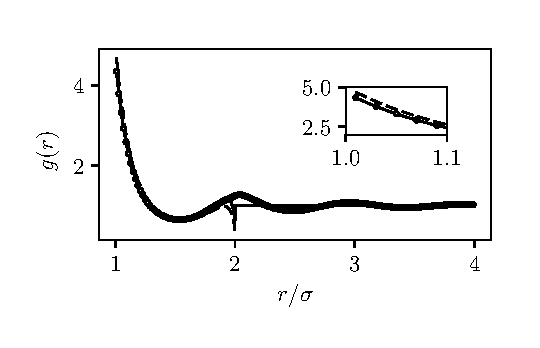
\includegraphics[width=\linewidth]{g2_phi045}
 \caption{$g^{(2)}(r)$ for $\eta = 0.45$.}
\end{SCfigure}

\subsection{Comparison with molecular dynamics simulations}
\subsection{Comparison with Kirkwood superposition approximation}

\ifdefined\includebibliography
  \printbibliography
\fi

\end{document}
